%%%%%%%%%%%%Loading Packages%%%%%%%%%%%%%%%%%%%%%%%%%%%%%%%
\documentclass{beamer}
\mode<presentation> \usetheme{Frankfurt}
\usepackage{hyperref}
\usepackage{rotating}
\usepackage{amsmath, amsthm, amssymb, amsfonts}
\usepackage{booktabs}
\usepackage[font=small, labelfont=bf]{caption}
%\setbeamercovered{transparent}
\usepackage{graphicx}
\usepackage{epsfig}
%\usepackage{tikz}
\usepackage{xcolor}
%\usepackage{emoji}
%\usepackage{colortbl}
\usepackage{caption}
\usepackage[svgnames]{xcolor}
\DeclareCaptionFont{myblue}{\color{RoyalBlue}}
\captionsetup{labelfont={myblue,bf}}
\setbeamertemplate{itemize items}[square]
\setbeamertemplate{footline}[frame number]

\newcommand{\x}[1]{\alert{#1}}
%\definecolor{darkblue}{RGB}{0,0,139} % Defining dark blue color
%\newcommand{\filledsquare}{\tikz \draw[fill=darkblue] (0,0) rectangle (0.2,0.2);}

\begin{document}
\title{A Statistician’s Experience}
\author{Abidemi K. Adeniji, PhD\\ResTORbio, Inc.\\
	\vspace{40pt} 
	Presented to\\
	NESS-NextGen Data Science Day\\
	Yale University\\
	New Haven, CT\\
	October 27, 2018}
	\date{}
\frame{\titlepage}

%%%%Discalaimer%%%%%%%%%%%%%%%%%%%%
\begin{frame}
	\frame{\frametitle{Disclaimer}}
	\centering\textbf{\underline{Disclamer}}\\
	The materials presented are solely the views of the presenter\\
	Abidemi K. Adeniji.
\end{frame}

%%%%%%%%%%%%% Creating overview (table of contents)%%%%%%%%%%%%%%%%%%%
\begin{frame}
\frametitle{Overview}
\tableofcontents[hideallsubsections]
\end{frame}

%%%%%%%%%%%First section%%%%%%%%%%%%%%%%%%%%%%%%%%%%%%
\section{Preparation}
\frame[plain,noframenumbering]{\frametitle{Outline}
\tableofcontents[currentsection, currentsubsection,hideallsubsections]}

%%%%%%%%%%%%%% First subsection for section one %%%%%%%%%%%%%%%%%%%%%%%%%%%%%%%%	
\subsection{School preparation}
\frame{\frametitle{Preparation}
	\tableofcontents[currentsection, currentsubsection]}

\begin{frame}
	\frame{\frametitle{School preparation}}
	\center
	\textbf{Public Speaking}\\
	\bigskip
	\begin{itemize}
		\item Actively seek opportunities to present.
		\begin{itemize}
			\item In group projects, ask to be the speaker.
		\end{itemize}
		\pause
		\item Learn how to tell your story.
	\end{itemize}	
\end{frame}


\begin{frame}
	\frame{\frametitle{School preparation}}
	\center
	\textbf{Public Speaking}\\
	\bigskip
	\begin{itemize}
		\item  Sign up for local clubs like Toastmasters
		\pause
			\begin{itemize}
				\item They are a leader in communication and leadership	development.
				\pause
				\item The bio-pharma market is changing, decisions are becoming
				more analytically driven giving statisticians more avenues for a
				sit at the table.
			\end{itemize}
	\end{itemize}
\end{frame}

\begin{frame}
	\frame{\frametitle{School preparation}}
	\center
	\textbf{Toastmasters locations in CT}
	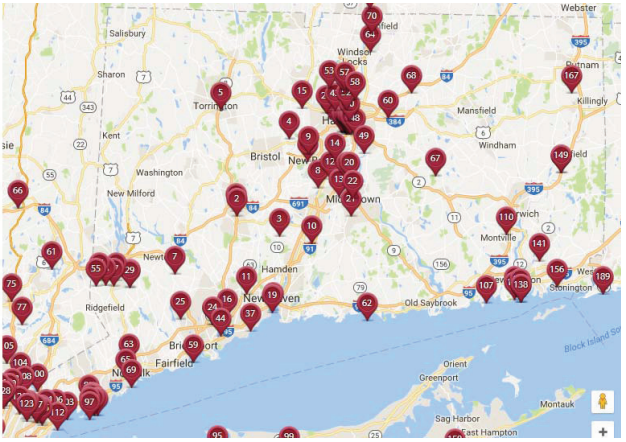
\includegraphics[width=0.85\textwidth]{toastmaster}
\end{frame}

\begin{frame}
	\frame{\frametitle{School preparation}}
	\center
	\textbf{Writing}\\
	\bigskip
	\begin{itemize}
		\item  Actively seek opportunities to write.
	\end{itemize}
	\pause
	\bigskip
	\textcolor{blue}{How to Write a Lot: A Practical Guide to Productive Academic
		Writing, P.J. Silvia, 2007}
\end{frame}

%%%%%%%%%%%%%% Second subsection for section one %%%%%%%%%%%%%%%%%%%%%%%%%%%%%%%%	
\subsection{Interview preparation}
\frame{\frametitle{Phone-screen interview}
	\tableofcontents[currentsection, currentsubsection]}
	
\begin{frame}
	\frame{\frametitle{Interview preparation}}
	\center
	\textbf{Recruiters}\\
	\pause
	\begin{itemize}
		\item  Recruiters can play an important role in getting you an interview.
		\pause
		\begin{itemize}
			\item However, understand that the job of the recruiter is not to get
			you a job,\pause \alert {but to fill a position.}
		\end{itemize}
	\end{itemize}
\end{frame}

\begin{frame}
	\frame{\frametitle{Interview preparation}}
	\center
	\textbf{Phone-screen interview}\\
	\pause
	\begin{itemize}
		\item Prepare as if you were at the on-site interview
		\pause
			\begin{itemize}
				\item If you plan to wear a suit for the potential on-site interview, do the same for the phone-screen interview (including shoes, tie, coat, watch, etc.).
				\pause
				\item Stand up during the call
			\end{itemize}
	\end{itemize}
\end{frame}
%%%%%%%%%%%%%%%%Second section%%%%%%%%%%%%%%%%%%%%%%%%%%%%%%%%%%%%%%%%%%%%%%%%%%%%%%
\section{On-site Interview}
\frame[plain,noframenumbering]{\frametitle{Outline}
	\tableofcontents[currentsection, currentsubsection]}

\begin{frame}
	\frame{\frametitle{On-site interview}}
	\center
	\textbf{On-site interview}\\
	\begin{itemize}
		\item Seek out university services to conduct mock interviews.
		\pause
		\item If possible obtain a copy of your interview schedule ahead of time and study your interviewers.
		\pause
		\item Know your resume!
		\pause
		\item Understand the job description and how \alert {you} plan to solve
		\alert {their} business needs.
		\pause
		\item Relax and have a conversation, be genuine in your approach
		to people.
		\pause
		\item If you dont know an answer, it’s better to admit a limited
		exposure to the topic, than to give a wrong answer.
	\end{itemize}
\end{frame}

\begin{frame}
	\frame{\frametitle{Mimic Octopus}}
		\begin{figure}
			\begin{center}
			\centering
	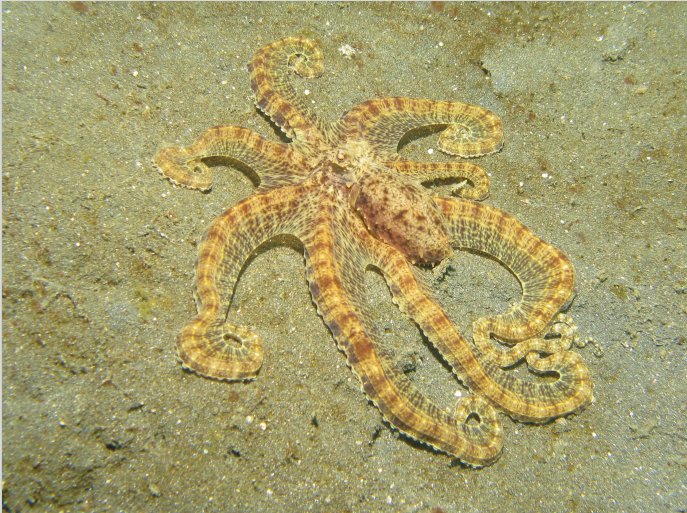
\includegraphics[width=0.80\textwidth]{octopus}
			\end{center}
	\caption {By Silke Baron from Vienna, Austria - Mimic Octopus, CC BY 2.0, https://commons.wikimedia.org/w/index.php?curid=11090270.}
		\end{figure}
\end{frame}

\begin{frame}
	\frame{\frametitle{On-site interview}}
	\center
	\textbf{Mimicking}\\
	\pause
	Mimicking - a way to connect with each interviewer
	\pause
	\begin{itemize}
	\item \alert{It is not about being fake, but about building a channel to
		communicate with each interviewer}
		\pause
			\begin{itemize}
			\item Interviewer is serious, I’m serious
			\pause
			\item Interviewer is joyous, I’m joyous
			\pause
			\item Interviewer talks about tennis, I talk about tennis 
\includegraphics[height=1em]{smiley-icon.png}
			\pause
			\item Interviewer sits upright, I sit upright	
			\end{itemize}
	\end{itemize}
\end{frame}

\begin{frame}
	\frame{\frametitle{Communication}}
	\center
	\underline{Communicating across functions}\\
	\vspace{15pt} 
	\begin{itemize}
		\item Communicate in simple terms, be confident, be humble
		\begin{itemize}	
		\item \textbf {“I couldn’t reduce it to the freshman level. That means
		we really don’t understand it”} - Richard Feynman
		\end{itemize}
	\end{itemize}
\end{frame}

\begin{frame}
	\frame{\frametitle{Communication}}
	\center
	Effective Meetings Training
\end{frame}

\begin{frame}
	\frame{\frametitle{Communication}}
	\center
	\underline{Holding Effective Meetings}\\
	\vspace{15pt} 
	\begin{itemize}
		\item 1st blinded report planning meeting (dissemination of data):
		leading efficient and effective meetings
	\end{itemize}
\end{frame}	

\begin{frame}
	\frame{\frametitle{ }}
	\center
	\textbf{Effective Meetings}\\
		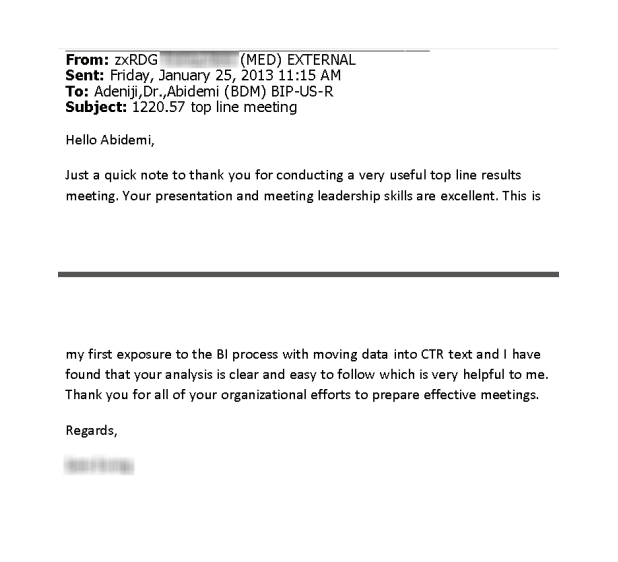
\includegraphics[width=0.80\textwidth]{effectiveness}
\end{frame}

\begin{frame}
	\frame{\frametitle{Thank You!}}
	\center
	Thank you for the opportunity to give this presentation.
\end{frame}

\end{document}